% % % % % % % % % % % % % % % % % % % % % % % % % % % % 
% mainintro.tex - Ian Huston
% $Id: mainintro.tex,v 1.57 2009/10/29 12:36:56 ith Exp $
% % % % % % % % % % % % % % % % % % % % % % % % % % % % 
% Redefine CVSRevision for this section
\renewcommand{\CVSrevision}{\version$Id: mainintro.tex,v 1.57 2009/10/29 12:36:56 ith Exp $}

% % % % % % % % % % % % % % % % % % % % % % % % % % % % % % % % 
% =========================================================== %
% % % % % % % % % % % % % % % % % % % % % % % % % % % % % % % % 
\chapter{Inflationary Cosmology}
\label{ch:introduction}
% % % % % % % % % % % % % % % % % % % % % % % % % % % % % % % % 
% =========================================================== %
% % % % % % % % % % % % % % % % % % % % % % % % % % % % % % % % 

In this chapter the foundations of inflationary cosmology are described. 
% 
In Section~\ref{sec:frw-intro} the
physics of
an isotropic and homogeneous universe is reviewed. The inflationary
scenario is introduced in Section~\ref{sec:inflation-intro}. 
First order cosmological perturbation theory is presented in
Section~\ref{sec:perts-intro} and inflationary models with non-canonical actions are
described in Section~\ref{sec:noncanoninfl}.
The current observational limits on inflationary models are outlined in
Section~\ref{sec:obs-intro} and departures from
Gaussian statistics are parametrised in Section~\ref{sec:fnl-intro}.

% Finally the structure and goals of the full thesis
% are described in Section~\ref{sec:goals-intro}.


% % % % % % % % % % % % % % % % % % % % % % % % % % % % % % % % 
% =========================================================== %
% % % % % % % % % % % % % % % % % % % % % % % % % % % % % % % % 
\section{The Friedmann-Robertson-Walker Universe}
\label{sec:frw-intro}
% % % % % % % % % % % % % % % % % % % % % % % % % % % % % % % % 
% =========================================================== %
% % % % % % % % % % % % % % % % % % % % % % % % % % % % % % % % 
The cosmological principle is central to the Friedmann-Robertson-Walker
(FRW\footnotemark) Universe. 
\footnotetext{Lema\^{i}tre is sometimes also included in this group to give
FLRW.}
According to this postulate there is no privileged
place in the universe and no privileged direction in which to make observations.
These assertions
are formalised by assuming that the universe is homogeneous and isotropic at
every point. This clearly conflicts with the highly inhomogeneous nature of matter
on planetary and solar system scales but is assumed to hold as larger and larger
scales are considered.
Surveys of the observable universe indicate that this holds up to the largest
scales observed \cite{Colless:2001gk, York:2000gk}. 
Historically homogeneity and isotropy were assumed primarily for simplicity.
Many alternative approaches can be taken. Violating these assumptions can
be done for example by specifying a preferred direction or supposing that the
universe is formed by a series of voids connected by filaments. Although many
of these approaches have been disregarded due to lack of evidence some are still
allowed by the observations
\cite{GarciaBellido:2008nz,Alexander:2007xx,Alnes:2005rw,Hunt:2008wp}.

This section outlines the dynamics of the standard Big Bang scenario.
By assuming homogeneity and isotropy the equations of motion of a
fluid-filled universe can be derived. What follows here is a
standard exposition of well-known physics and has been the subject of
numerous reviews including Refs~\cite{book:kolbturner, book:kip, book:liddle}.


By imposing both homogeneity and isotropy on a general 4-dimensional metric, the
line element $\d s^2$ of the FRW universe with coordinates $(t,r,\theta,\omega)$
is obtained:
% 
\begin{equation}
 \label{eq:frwmetric-intro}
\d s^2 = -\d t^2 + a^2(t)
  \left( 
    \frac{\d r^2}{1-Kr^2} + r^2\left(\d\theta^2 + \sin^2(\theta)
\d\omega^2\right)
  \right)\,,
\end{equation}
% 
where $K=+1, 0$ or $-1$ depending on whether the universe is closed, flat
or open respectively. The time-like coordinate in the metric is $t$, known as
proper time, and differentiation with respect to $t$ is denoted by an
overdot $(\dot{~})$. 


The spatial part of the FRW metric is multiplied by the scale factor $a(t)$.
This characterises the size of space-like hypersurfaces at
different coordinate times. In an expanding universe $a$ grows with
increasing $t$ and
$\dot{a}>0$.
The definition of the Hubble parameter $H$ captures this expansion:
% Definition of Hubble parameter
\begin{equation}
 \label{eq:Hdefn-intro}
  H = \frac{\dot{a}}{a} \,.
\end{equation}
%


The Einstein equations can be derived by the variational principle from the
action $S$ where $S\equiv S_\mathrm{EH} + S_\mathrm{M}$. This is the sum
of the
Einstein-Hilbert ($S_\mathrm{EH}$) and matter ($S_\mathrm{M}$) actions which are
defined as 
% 
\begin{eqnarray}
\label{eq:EHeqn-intro}
 S_\mathrm{EH} &=& \frac{1}{16\pi G}\int \d^4 x \sqrt{|g|} \left(R +
2\Lambda_c\right) \,,\\
\label{eq:matteraction-intro}
 S_\mathrm{M} &=& \int \d^4 x \sqrt{|g|}
\mathcal{L}_\mathrm{M} \,.
\end{eqnarray}
%
Here $g$ is the determinant of the metric $g_{\mu\nu}$, $R$ is the Ricci
scalar, $G$ is Newton's gravitational constant, $\Lambda_c$ is a cosmological
constant term 
and $\mathcal{L}_\mathrm{M}$ is the sum of the Lagrangian densities
for all the matter fields.
Changing either the matter or gravity actions will affect the
resultant physics. In this work we focus our attention only on the matter
Lagrangian and will use the standard Einstein-Hilbert action throughout.
We can now write down the Einstein equations for a general matter Lagrangian:
% 
\begin{equation}
\label{eq:einstein-intro}
 R_{\mu\nu} - \frac{1}{2}R g_{\mu\nu} = 8\pi G T_{\mu\nu} + \Lambda_c
g_{\mu\nu}\,,
\end{equation}
% 
where $T_{\mu\nu}$ is the stress energy tensor obtained by the variation of the
matter Lagrangian. 
In the definitions above we have included a
cosmological constant term, $\Lambda_c$, for completeness. In the early
universe this term is subdominant and will be negligible until much later
\cite{book:liddle}. From now on we will
disregard the contribution of such a term in the early universe.


We concentrate now on the case of a universe filled with a perfect
fluid. Suppose $u^\mu$ is the 4-velocity of this fluid with $u^\mu
u_\mu=-1$. The stress-energy tensor of the fluid is
% 
\begin{equation}
 \label{eq:fluidstress-intro}
  T^\mu_{~\nu} = (E + P)u^\mu u_\nu + P\delta^\mu_\nu \,,
\end{equation}
% 
where $E$ is the matter energy density and $P$ is the isotropic pressure.
The trace of $T$ is given by
% 
\begin{equation}
 \label{eq:Ttrace-intro}
  T^\mu_{~\mu} = -E + 3P\,.
\end{equation}
% 
The Einstein equations and the stress-energy tensor of the
perfect fluid can now be used to derive the equations of motion of the fluid.
From the metric in \eq{eq:frwmetric-intro} the $00$ and $ij$ components of the
Ricci tensor can be found:
% 
\begin{eqnarray}
\label{eq:Ricci00-intro}
 R_{00} &=& -3 \frac{\ddot{a}}{a} \,,\\
\label{eq:Ricciij-intro}
 R_{ij} &=& \delta_{ij} \left[ 2\dot{a}^2 +
  a \ddot{a} + 2\frac{K}{a^2} \right] \,.
\end{eqnarray}
% 
The Friedmann equations are then determined from the Einstein equations
\eqref{eq:einstein-intro}.
The $00$ equation gives
% 
\begin{equation}
 \label{eq:Friedmann1-intro}
 H^2 = \left(\frac{\dot{a}}{a}\right)^2 = \frac{8\pi G}{3} E - \frac{K}{a^2}\,,
\end{equation}
% 
while the trace of the Einstein equations gives the Raychaudhuri or
acceleration equation
% 
\begin{equation}
 \label{eq:Friedmann2-intro}
 \frac{\ddot{a}}{a}  = -\frac{4\pi G}{3}(E + 3P)\,.
\end{equation}
% 
By combining these two equations we can determine a continuity equation for the
energy density:
\begin{equation}
 \label{eq:continuity-intro}
 \dot{E} + 3H(E+P) = 0 \,.
\end{equation}


The last three equations \eqref{eq:Friedmann1-intro},
\eqref{eq:Friedmann2-intro}
and \eqref{eq:continuity-intro} will determine the evolution of the
perfect fluid. Two important solutions of these equations are
the radiation and
matter dominated universes. In the standard Big Bang scenario the universe is
dominated by radiation to a good approximation until matter becomes dominant
at later times \cite{book:kolbturner}. These different components
change the rate of expansion
of the universe. For relativistic radiation $P_\mathrm{rad}=E_\mathrm{rad}/3$
and integrating the continuity equation \eqref{eq:continuity-intro} gives
$E_\mathrm{rad}\propto a^{-4}$. Matter conversely is taken to be dust-like with
zero
pressure and so $E_\mathrm{matter}\propto a^{-3}$. The dependence of $a$ on $t$
can then be
found from \eq{eq:Friedmann1-intro}, giving $a\propto t^{1/2}$ and $a\propto
t^{2/3}$ for the radiation and matter eras respectively.


% Horizons
Instead of using coordinate time as above we could bring
the scale factor outside the whole metric and use conformal time $\eta$
defined by
% Conformal time
\begin{equation}
\label{eq:etatime-intro}
 \eta = \int\frac{\d t}{a}\,.
\end{equation}
A prime ($'$) signifies differentiation with respect to $\eta$. 
The metric written in conformal time is then 
% 
\begin{equation}
 \label{eq:frwconformal-intro}
\d s^2 = a^2(t)
  \left( -\d\eta^2 +
    \frac{\d r^2}{1-Kr^2} + r^2\left(\d\theta^2 + \sin^2(\theta)
\d\omega^2\right)
  \right)\,,
\end{equation}

% 
Because all the coordinates in the line element are now scaled by $a(t)$ we
have defined a coordinate grid which does not change as the universe expands.
These ``comoving'' coordinates allow distances to be compared at different
eras with ease. A comoving distance $x$ can be translated into a physical
distance $d$ by
% 
\begin{equation}
 \label{eq:comovingdefn-intro}
 d = ax \,.
\end{equation}
The physical distance changes as the universe expands but the comoving distance
will remain fixed. 

One particularly important distance is the maximum distance light could have
propagated from some initial time $t_i$ to a later time $t$. From
\eq{eq:comovingdefn-intro} this is simply the conformal time integrated from
the initial time and is called the comoving or particle horizon.
If the initial time is restricted to
being at some finite time in the past, as in the Big Bang scenario, then the
particle horizon will be finite. Two points which are further apart than
this finite distance could never have been in causal contact. This
is the origin of one of the major problems with the standard Big Bang scenario
and will be discussed in the next section.
Rewriting the comoving horizon as
% 
\begin{equation}
 \eta = \int_{a_i}^a \frac{\d a'}{a'} \frac{1}{a' H(a')} \,,
\end{equation}
shows that it is also the logarithmic integral of the comoving Hubble
radius $1/aH$. This distance is how far particles can travel in one
``e-folding'', the time for $a$ to expand by one exponential factor. 
The number of e-foldings between two measurements of the scale factor, $a_i$
and $a_f$ is given by
\begin{equation}
\label{eq:nefolddefn-intro}
 \N = \ln \frac{a_f}{a_i}\,.
\end{equation}

Particles
that are separated by more than the Hubble radius cannot be in causal
contact now. Particles separated by more than the
comoving horizon, however, could never have been in causal contact. In addition
to the Hubble parameter $H$, it will be useful
to define the parameter $\H = aH = a'/a$. The comoving Hubble radius is then
$1/\H$.







% % % % % % % % % % % % % % % % % % % % % % % % % % % % % % % % 
% =========================================================== %
% % % % % % % % % % % % % % % % % % % % % % % % % % % % % % % % 
\section{Inflation}
\label{sec:inflation-intro}
% % % % % % % % % % % % % % % % % % % % % % % % % % % % % % % % 
% =========================================================== %
% % % % % % % % % % % % % % % % % % % % % % % % % % % % % % % % 
In this section we introduce the inflationary scenario. First we briefly
describe how it solves two major problems with the standard Big Bang
picture: the flatness problem and the horizon problem \cite{book:liddle}. We go on to
describe canonical slow-roll inflation, the generation of
perturbations from quantum fluctuations and inflation from non-canonical
actions.

\subsection{Problems with the Big Bang scenario}
Although remarkably successful in describing the evolution of the universe from
very early in its history, the standard Big Bang scenario suffers from a number
of serious problems. Two of the main problems are described in this section.

\subsubsection{Flatness Problem} 
\label{sec:flatprob}
The Friedmann equation
\eq{eq:Friedmann1-intro} can be re-written as
% 
\begin{equation}
\label{eq:omegadefn-intro}
\Omega(t) - 1 = \frac{K}{(aH)^2} = \frac{K}{\dot{a}^2} \,,
\end{equation}
% 
where $\Omega(t)=E(t)/E_\mathrm{crit}$ and the critical density
$E_\mathrm{crit}= 3H^2/8\pi G$. 
If $\ddot{a}>0$ then $\Omega$ goes towards the critical value $\Omega=1$, whereas if
$\ddot{a}<0$ it is diverges from this value. The flat universe, $K=0$,
is an unstable fixed point in the parameter space.
Current observations confirm $\Omega=1$ within about 2\% at a 95\% confidence
level \cite{Komatsu:2008hk}.
During the radiation and matter dominated eras $aH$ is decreasing with time,
meaning that $\Omega$ diverges away from 1. If it is measured now as being very
close to 1 then in the past it must have been even closer. The requirement of
extreme proximity to $\Omega=1$ as an initial condition is known as the
flatness problem. 


\subsubsection{Horizon Problem} \label{sec:horizprob}
The particle horizon, also known
as the comoving horizon, defines the maximum separation between two points that
have been in causal contact sometime in the past. During the radiation and
matter eras this comoving horizon increases monotonically and so length-scales
which are now entering the horizon would have been far outside the horizon in
the past. 
The CMB as observed by the WMAP satellite is extremely smooth on scales that
would have been far outside the horizon at the time of last scattering
\cite{Komatsu:2008hk}. These regions of space have very similar energies and
yet they could not have been in causal contact since the Big Bang. 

% 
% \subsubsection{Cosmological Defects} \label{sec:cosdefects}
% The Big Bang achieved temperatures at which a Grand Unified Theory
% (GUT) would predict a higher order symmetry gauge group \cite{book:kolbturner}.
% During cooling,
% spontaneous symmetry breaking could leave relics that might survive to
% the current day. Magnetic monopoles, cosmic strings and domain walls are some of
% the unwanted features predicted by GUT models. However, none of these features
% have been observed and some mechanism is needed to explain their absence.
% 



% % % % % % % % % % % % % % % % % % % % % % % % % % % % % % % % 
% =========================================================== %
% % % % % % % % % % % % % % % % % % % % % % % % % % % % % % % % 
\subsection{Inflation and Canonical Slow-roll}
\label{sec:slowroll-intro}
% % % % % % % % % % % % % % % % % % % % % % % % % % % % % % % % 
% =========================================================== %
% % % % % % % % % % % % % % % % % % % % % % % % % % % % % % % % 

Inflation is a period of accelerated expansion in the size of the universe
which took place just after the Big Bang
\cite{Starobinsky:1980te,Guth:1980zm,Albrecht:1982wi,Linde:1981mu,
Starobinsky:1982ee}. During this
expansion the comoving Hubble radius $(aH)^{-1}$ decreases and the isotropic
pressure of the universe is negative \cite{book:liddle, Baumann2009}:
% 
\begin{equation}
\label{eq:infldefn-intro}
 \frac{\d }{\d t}\left( \frac{1}{aH}\right) <0 \Rightarrow \ddot{a}>0
  \Rightarrow E + 3P < 0 \,.
\end{equation}
% 
We can also define a new parameter 
% 
\begin{equation}
\label{eq:epsilonHdefn-intro}
\varepsilon_H = -\frac{\dot{H}}{H^2}\,,
\end{equation}
% 
and then rewrite
the Raychaudhuri equation \eqref{eq:Friedmann2-intro} as
% 
\begin{equation}
 \label{eq:Friedeps-intro}
 \frac{\ddot{a}}{a} = H^2 (1-\varepsilon_H)\,.
\end{equation}
% 
This parametrisation means that inflation only occurs when $\varepsilon_H<1$.
In this subsection we describe briefly how inflation solves the problems
outlined above and outline the inflationary dynamics of single scalar field
models. 

Both the horizon and flatness problems described above are statements about our
reluctance to impose fine-tuned initial conditions. Inflation removes the need
to fix these conditions at the start of the Big Bang.
A period of decreasing Hubble radius before the radiation period could explain the
homogeneity of temperatures in the CMB at large scales.
Comoving scales that entered the horizon recently, such as
those we observe in the CMB, would have been within the horizon previously. 
During this period, the energy density could reach an equilibrium
value.
Figure~\ref{fig:comovingscales-intro} shows how by extending
the era of inflation far enough into the past any comoving length could
previously have been inside the horizon.
Observations require that inflation lasted at least long enough that all the
scales we measure today were previously inside the horizon. 
% 
\begin{figure}
 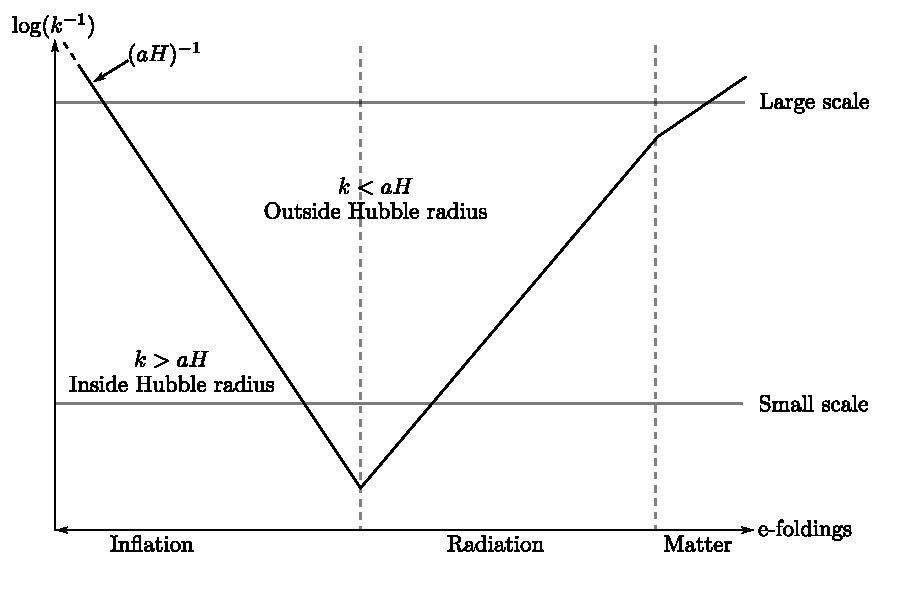
\includegraphics[width=\textwidth]{graphs/scales.pdf}
 \caption[Comoving scales and the Hubble radius]{Comoving scales that have recently
entered the horizon would
previously have been inside the horizon if the inflationary period extended far
enough into the past.}
 \label{fig:comovingscales-intro}
\end{figure}
% 

Now consider the time derivative of $|\Omega -1|$ as defined in
\eq{eq:omegadefn-intro}:
% 
\begin{equation}
 \label{eq:omegaderiv-intro}
 \frac{\d}{\d t}\left(|\Omega -1 |\right) = 2\frac{\d}{\d t}
\left(\frac{1}{aH}\right)\,.
\end{equation}
% 
If the universe is not flat to begin with, a period of inflation of sufficient
duration will push it
towards $\Omega=1$, solving the flatness problem. Instead of an unstable point
in the parameter space, $\Omega=1$ is an attractor during the inflationary
phase. 
% 

To solve the horizon and flatness problems the duration of the inflationary era
must be
sufficiently long. Approximately $50$--$70$ e-foldings is considered standard
\cite{book:liddle}. Inflation
can last longer than this but only the last 50--70 e-foldings will be important
for the length scales of our observable universe. As the scale factor of the
universe expands
in the region of $e^{60}\simeq 10^{26}$ times, the volume would increase by a
factor of $e^{180}$.  The number density
of any monopoles or other relics that existed before inflation would therefore be
diluted so much that observing these relics would be increasingly unlikely. 


As mentioned above during inflation the universe is filled with material that
has negative isotropic pressure.
Clearly whatever drives inflation cannot be matter or radiation in their usual
forms. The simplest proposal is to fill the universe with a single scalar field
$\varphi$. The canonical action for this field is
\begin{equation}
\label{eq:phiaction-intro}
 \mathcal{L}_\mathrm{M} \equiv P(\varphi, X) = X -V(\varphi) \,,
\end{equation}
where $X=-\frac{1}{2}g_{\mu\nu}\partial^\mu\varphi \partial^\nu\varphi$ denotes
the kinetic energy of $\varphi$, $V(\vp)$ is the potential and $P(\varphi, X)$
is called the kinetic
function. In Section~\ref{sec:noncanoninfl} we will consider other
choices for $P$. 

The equation of motion for $\varphi$ for the canonical $P=X-V$ is
% 
\begin{equation}
 \label{eq:phieom1-intro}
 \ddot{\vp} + 3H\dot{\vp} -\nabla^2 \vp + \frac{\delta V}{\delta \vp} = 0\,.
\end{equation}
% 
If we now restrict ourselves to considering the homogeneous part of the field,
$\vp=\vp(t)$, the $\nabla^2\vp$ term disappears and the functional derivative
of $V$ becomes a standard derivative $V_{,\vp}$. 
% A subscripted comma will
% denote partial differentiation, $V_{,\vp}=\partial V/\partial\vp$.
With these choices we have the following relations for the matter
energy-density and isotropic pressure:
% 
\begin{eqnarray}
\label{eq:EandP-intro}
 E &=& \frac{1}{2}\dot{\varphi}^2 + V(\varphi) \,,\\
\label{eq:Pdefn-intro}
 P &=& \frac{1}{2}\dot{\varphi}^2 - V(\varphi) \,.
\end{eqnarray}
% 
Under these conditions the kinetic function $P(\varphi, X)$ can be identified as
the isotropic pressure. The dynamics of the field are governed by the potential
$V(\varphi)$. Inflation requires $P<-E/3$ so from Eqs \eqref{eq:EandP-intro} and
\eqref{eq:Pdefn-intro} inflation
can also be thought of as a period when the potential energy $V$ dominates over
the kinetic energy. 


Inflation needs to last long enough to solve the problems described above. A generic
potential is not likely to satisfy these requirements without fine-tuning. One
approach to achieve this longevity is to require potentials to meet
conditions under which the inflationary period is necessarily long. 

We have seen that for
inflation to occur the potential needs to dominate over kinetic energy. From
\eq{eq:EandP-intro} this occurs in the limit $P\rightarrow -E$ or equivalently
$\varepsilon_H \ll 1$. However for this to remain the case for a sufficiently long
period the second derivative of $\vp$ must be small enough. If we define
another parameter 
% 
\begin{equation}
 \label{eq:etaHdefn-intro}
 \eta_H \equiv -\frac{\d \ln \dot{\vp}}{\d \ln a} =
-\frac{\ddot{\vp}}{H\dot{\vp}}
 =\varepsilon_H -\frac{\dot{\varepsilon_H}}{2H\varepsilon_H}\,,
\end{equation}
% 
then taking $|\eta_H|\ll 1$ will ensure that $\dot{\vp}$ and $\varepsilon_H$
change slowly, allowing inflation to last longer.

The approximations $\varepsilon_H\ll 1$ and $|\eta|\ll 1$ are known as the
slow-roll conditions because they force the inflaton field $\vp$ to roll down
the potential $V$ slowly. The parameters $\varepsilon_H$ and $\eta_H$ are known as
slow-roll parameters. Setting $\ddot{\vp}$ to be small is equivalent to
making the friction $H\dot{\vp}$ in \eq{eq:phieom1-intro} dominant. With
these approximations the
equations of motion for a slowly rolling field become
% 
\begin{eqnarray}
 \dot{\vp} &\simeq& - \frac{V_{,\vp}}{3H}\,, \\
 H^2 &\simeq& \frac{8\pi G}{3}V(\vp)\,.
\end{eqnarray}




% % % % % % % % % % % % % % % % % % % % % % % % % % % % % % % % 
% =========================================================== %
% % % % % % % % % % % % % % % % % % % % % % % % % % % % % % % % 
\section{Perturbations}
\label{sec:perts-intro}
% % % % % % % % % % % % % % % % % % % % % % % % % % % % % % % % 
% =========================================================== %
% % % % % % % % % % % % % % % % % % % % % % % % % % % % % % % % 

We considered a homogeneous scalar field in the analysis of
Section~\ref{sec:inflation-intro}. Such a field, however, will
lead only to a homogeneous universe later. How does the myriad structure
that we see around us form? From stars to galaxies to clusters, the
gravitational force has concentrated energy density over the history of the
universe but some initial fluctuation must have been present to begin this
process. One of the main achievements of inflation is to provide a physical
origin for
such initial fluctuations. In Chapter~\ref{ch:perts} we will formally develop
cosmological perturbation theory up to second order. In this section we 
review first order perturbation theory and introduce the observable quantities
important for inflation.


Suppose that a full inhomogeneous scalar field
$\varphi$ is split into a homogeneous background field $\vp_0$ as we described
above and an inhomogeneous perturbation $\dvp{}(\eta,x^i)$ for $i=1,2,3$. For the
following
analysis to be valid the perturbation must be much smaller than the background
field value. From the amplitude of perturbations in the CMB this approximation
can be seen to be valid \cite{Komatsu:2008hk}. 

If we suppose that $\epsilon$ is a small quantity then the split in $\vp$
can be written as \cite{Malik:2008im}
% 
\begin{equation}
\label{eq:pertsplit-intro}
\vp(\eta, x^i) = \vp_0(\eta) + \epsilon\dvp{}(\eta, x^i) \,.
\end{equation}
% 
 The perturbation $\dvp{}(\eta, x^i)$ can be further expanded in
powers of $\epsilon$.  We will follow the
custom of not explicitly writing $\epsilon$, instead relying on the order of
the perturbation, denoted by a subscript, to keep track.
If we expand in a Taylor series then up to second order (\ie including terms
up to $\epsilon^2$) we have:
% 
\begin{equation}
 \vp(\eta, x^i) = \vp_0(\eta) + \dvp1(\eta, x^i) + \frac{1}{2}\dvp2(\eta, x^i)
\,.
\end{equation}
% 
There is some freedom in how the split of the perturbations into different
orders is made. We will suppose that the first order perturbation $\dvp1$
contains only linear contributions and the higher order terms contain non-linear
terms. 


Instead of working in coordinate space we can also consider
the perturbation in Fourier space using the definition
% 
\begin{equation}
\label{eq:fourierdefn-intro}
 \dvp{}(\eta, x^i) = \frac{1}{(2 \pi)^3} \int \d^3k \dvp{}(\kvi) \exp (i k_i
x^i)
\,,
\end{equation}
where $k^i$ are the components of the comoving wavenumber vector $\bf{k}$. The
amplitude of this
vector $k=|\kvi|$ identifies whether a particular mode is inside or outside
the comoving horizon. Wavemodes inside the comoving horizon are identified by
$k>aH$ while $k<aH$ for those outside the horizon. 


We must also consider perturbations in the metric tensor $g_{\mu\nu}$. If the
background metric is the FRW one described in Section~\ref{sec:frw-intro} then
the metric can be written with perturbations, up to first order, as follows:
% 
\begin{align}
 \label{eq:pertmetric-intro}
 g_{00} &= -a^2 (1 + 2\phi_1) \,, \nonumber\\
 g_{0i} &= a^2 (B_{1,i} - S_{1i}) \,, \nonumber\\
 g_{ij} &= a^2\left[ (1 - 2\psi_1)\delta_{ij} + 2E_{1,ij} + 2F_{1(i,j)} +
h_{1ij}
\right] \,.
\end{align}
% 
The vectors $S_{1i}$ and $F_{1i}$ are divergence free and the tensor part
$h_{1ij}$
is divergence free and traceless:
% 
\begin{equation}
 S^k_{1~,k} = 0\,, \quad F^k_{1~,k}=0\,; \qquad h^{ik}_{1~~,k} = 0\,,
  \quad h^k_{1~k}= 0\,.
\end{equation}
% 
In the previous equation $\phi$ is the lapse function, $\psi$ is the curvature
perturbation, $B$ and $E$ are the scalar part of the shear, $S_i$, and $F_i$
are the vector parts of the shear, and $h_{ij}$ is the tensor perturbation
describing gravitational waves.
% Scalar field inflation does not produce vector perturbations so we will not
% consider them  \cite{book:liddle}.


Splitting an inhomogeneous spacetime into background and perturbation is not a
covariant operation. This leads to an ambiguity in the choice of coordinates
which must be rectified by choosing a gauge. Gauge transformations relate
physical results in one gauge to those in another. To choose a gauge one must
specify how spacetime is foliated, i.e. a slicing, and how coordinates in one
spatial hypersurface are related to those in another, i.e. a threading
\cite{Malik:2008im}. We will
employ the uniform curvature gauge in which spatial hypersurfaces are flat. It
is also known as the flat gauge.

The gauge transformation vector at first order  $\xi_1^\mu$ can be split into
scalar
and vector parts
% 
\begin{equation}
\label{eq:xidefn-intro}
 \xi_1^\mu = (\alpha_1, \beta_{1,}^{~i} + \gamma_1^i)\,,
\end{equation}
% 
where the vector part obeys $\gamma_{1~,k}^{~k}=0$. A scalar quantity such as
the inflaton perturbation will transform as \cite{Malik:2008im, Malik:2008yp}
% 
\begin{equation}
 \label{eq:dphitransform-intro}
 \wt{\dvp1} = \dvp1 + \vp_0' \alpha_1\,,
\end{equation}
where a tilde ($\wt{~}$) denotes a transformed quantity. For the metric
perturbations the
transformations for the scalars are
\begin{eqnarray}
 \label{transphi1}
\widetilde {\phi_1} &=& \phi_1 +\H\alpha_1+\alpha_1'\,,\\
%
\label{transpsi1}
\widetilde \psi_1 &=& \psi_1-\H\alpha_1 \,,\\
%
\label{transB1}
\widetilde B_1 &=& B_1-\alpha_1+\beta_1'\,,\\
%
\label{transE1}
\widetilde E_1 &=& E_1+\beta_1\,,
\end{eqnarray}
and for the vectors
\begin{eqnarray}
 \label{transS1}
\widetilde {S_{1}^{~i}} &=& S_{1}^{~i}-\gamma_1'\,, \\
%
\label{transF1}
\widetilde {F_{1}^{~i}} &=& F_{1}^{~i}+\gamma_1\,. 
\end{eqnarray}
% 
The tensor perturbation $h_{1ij}$ does not change under transformation at first
order, but does at subsequent orders.
The flat gauge, which we will use, is the one in which spatial hypersurfaces
are not perturbed by scalar or vector perturbations, so $\wt{\psi_1} = \wt{E_1}
=0$ and $\wt{F_{1i}} = \textbf{0}$.  This is equivalent to the transformation
% 
\begin{equation}
 \alpha_1 = \frac{\psi_1}{\H}\,,\quad \beta_1=E_1 \,, \quad \gamma^i_1 =
-F^i_1\,.
\end{equation}

A gauge invariant inflaton perturbation variable is the Sasaki-Mukhanov
variable \cite{Mukhanov:1990me, Mukhanov:1988jd,
Sasaki:1986hm}:
% 
\begin{equation}
\label{eq:flatdvp1-intro}
 \wt{\dvp1} \equiv \dvp1 + \vp_0'\frac{\psi_1}{\H}\,,
\end{equation}
% 
In the flat gauge this is just $\dvp1$. We will work in flat
gauge from now on and so will drop the tildes on quantities in that gauge.

Another very important gauge invariant quantity is the comoving curvature
perturbation $\R$. At first order in the flat gauge $\R$ is related to the
inflaton perturbation by \cite{Malik:2008im}
% 
\begin{equation}
\label{eq:flatRdefn-intro}
 \R = \frac{\H}{\vp_0'}\dvp1\,.
\end{equation}
% 
We are interested in the power spectrum of the curvature perturbation as this
is directly related to the temperature fluctuations that we can observe in the
CMB. 

The action \eqref{eq:phiaction-intro},
including perturbations of $\vp$ and $g_{\mu\nu}$ up to first order, is
varied to get the equation of motion of $\dvp1$. 
In the flat gauge the equation can be rewritten in terms of the inflaton field
values only by eliminating the metric perturbations using
\eq{eq:flatdvp1-intro}. 
% 
In Fourier space and in terms of the conformal time $\eta$, the closed form of
the first order perturbation equation of motion is \cite{Malik:2008im}
% 
\begin{eqnarray}
\label{eq:fokg-intro}
&& \dvp1''(\kvi) + 2\H \dvp1'(\kvi) + k^2\dvp1(\kvi) \nonumber\\
&&+ a^2 \left[\Upp +
\frac{8\pi G}{\H}\left(2\vp_{0}' \Uphi + (\vp_{0}')^2\frac{8\pi G
}{\H}\U\right)\right]\dvp1(\kvi) = 0 \,,
\end{eqnarray}
% 
where $\U$ is the background value of the potential $V(\vp)$.
%
% \addtodo{Check that the Mukhanov eqn is equivalent} 
% If we know assume that $\varepsilon_H \ll1 $ and $|\eta_H|\ll1$ then we get the
% slow-roll form of this equation:
% % 
% \begin{equation}
%  \label{eq:fokg-sr-intro}
%  \dvp1''(\kvi) + 2\H \dvp1'(\kvi) + \left( k^2 + a^2\Upp\right) \dvp1(\kvi) =
% 0 \,.
% \end{equation}


Substituting $u=a\dvp1$ gives the Mukhanov equation \cite{Mukhanov:1990me}
% 
\begin{equation}
 \label{eq:ueq-intro}
 u''(\kvi) + \left[ k^2 -\frac{z''}{z}\right]u(\kvi) = 0\,,
\end{equation}
% 
where $z= a\vp_0'/\H$.

\subsection{Quantum perturbations}
So far we have considered classical perturbations. The generation of
fluctuations is a quantum effect, however, and we need to consider the
perturbations as quantum operators in some vacuum. 

In Minkowski space the quantisation of $u(\kvi)$ is straightforward.
The perturbation modes can be written in terms of quantum operators as
% 
\begin{equation}
 u(\kvi)\rightarrow\hat{u}(\kvi) = 
  w(\kvi) \hat{a}(\kvi) + w^\star(-\kvi)\hat{a}^\dagger(-\kvi) \,.
\end{equation}
%
The mode function $w(\kvi)$ obeys the same equation of motion as $u(\kvi)$:
% 
\begin{equation}
\label{eq:weqn-intro}
 w''(\kvi) + \left[ k^2 -\frac{z''}{a}\right]w(\kvi) = 0\,.
\end{equation}
% 
The operators $\hat{a}^\dagger$ and $\hat{a}$ are the usual creation and
annihilation operators. They act on quantum states by adding or
removing particles. The zero particle vacuum state, $|0\rangle$, is such that
% 
\begin{equation}
 \hat{a}^\dagger|0\rangle = |1\rangle\,,\quad \hat{a}|0\rangle = 0\,.
\end{equation}
% 
In Minkowski space these operators have the usual commutation relations
% 
\begin{equation}
 [\hat{a}(\kb), \hat{a}^\dagger(\kb')] = (2\pi)^3 \delta(\kb -\kb') \\
\end{equation}
and
\begin{equation}
[\hat{a}(\kb), \hat{a}(\kb')] = 0\,.
\end{equation}
% 
The $w$ modes are normalised by the condition \cite{Mukhanov:2005sc}
% 
\begin{equation}
\label{eq:quantcondition-intro}
 i(w^\star(\kvi)w'(\kvi) - {w^{\star}}'(\kvi)w(\kvi)) = 1\,.
\end{equation}


In the expanding FRW background the choice of vacuum is not straightforward.
Suppose one observer selects a zero particle state as the vacuum. Another
observer accelerating with respect to the first will see particles being
created in this ``vacuum'' state due to the Unruh effect
\cite{Kinney2009, Unruh1976a}. In selecting the vacuum we must choose one of the
many equivalent options.
To do this we consider the far past where $\eta\rightarrow -\infty$. The wavelengths of all the
modes are then much smaller than the Hubble radius and curvature scale. The modes are
therefore assumed to evolve in flat space. This suggests the Minkowski vacuum as the
most natural vacuum state to select and this choice of vacuum at
early times is known as the Bunch-Davies vacuum.
% 
In the limit $\eta\rightarrow -\infty, k/aH\rightarrow \infty$ the mode equation
\eq{eq:weqn-intro} becomes
% 
\begin{equation}
  w''(\kvi) + k^2 w(\kvi) = 0\,,
\end{equation}
% 
which has the plane wave solution
% 
\begin{equation}
\label{eq:subhsoln-intro}
 w(\kvi) = \frac{1}{\sqrt{2k}} e^{-ik\eta}\,.
\end{equation}
% 
This is the initial condition for modes which are well inside the horizon.

Now consider the de Sitter limit in which $\varepsilon_H\rightarrow 0$ and $H$
is constant. We have $z''/z = a''/a = 2/\eta^2$ so the mode equation is
% 
\begin{equation}
  w''(\kvi) + \left[ k^2 -\frac{2}{\eta^2} \right]w(\kvi) = 0\,.
\end{equation}
% 
A full general solution for $w$ is
% 
\begin{equation}
 w(\kvi) = A\frac{e^{-ik\eta}}{\sqrt{2k}}\left(1 -\frac{i}{k\eta}\right)
	  +B\frac{e^{+ik\eta}}{\sqrt{2k}}\left(1 +\frac{i}{k\eta}\right)\,.
\end{equation}
% 
Taking the condition \eqref{eq:quantcondition-intro} along with the solution
for subhorizon modes in \eq{eq:subhsoln-intro} we find that $A=1$ and $B=0$.
Thus the full solution in de Sitter space is \cite{book:liddle}
% 
\begin{equation}
\label{eq:wfinal-intro}
 w(\kvi) = \frac{e^{-ik\eta}}{\sqrt{2k}}\left(1 -\frac{i}{k\eta}\right)\,.
\end{equation}
% 
Inflation in spacetimes that are close to de Sitter will contain perturbations
with a spectrum defined by \eq{eq:wfinal-intro}. The slow-roll approximation is
enough to ensure that inflation occurs in a quasi-de Sitter spacetime.
However, the initial conditions for Fourier modes in \eq{eq:subhsoln-intro}
apply to non slow-roll models so long as they are applied well before horizon
crossing.


\subsection{Power spectra and spectral indices}
The power spectrum of the inflaton perturbation $\dvp1 = u/a$ can now be
defined as
% 
\begin{equation}
  \langle \dvp1(\textbf{k}) \dvp1(\textbf{k}') \rangle 
   \equiv (2\pi)^3 \delta(\textbf{k} + \textbf{k}') P_{\dvp{}}^2 (k)
   = (2\pi)^3 \delta(\textbf{k} + \textbf{k}') \frac{|w(\kb)|^2}{a^2}\,,
\end{equation}
% 
where $\langle \ldots \rangle$ denotes the ensemble average. 
If taken over a large enough volume the ensemble average and spatial average
are equivalent \cite{book:lyth}.
The power spectrum
$P_{\dvp{}}^2$ depends only on the magnitude of the wavenumber
vector $k=|\bf{k}|$ but has dimensions of $k^{-3}$. A dimensionless power
spectrum
can be defined as
% 
\begin{equation}
 \label{eq:curlPrdefn-intro}
 \mathcal{P}_{\dvp{}}^2= \Delta^2_{\dvp{}} \equiv \frac{k^3}{2\pi^2}
P_{\dvp{}}^2(k)\,.
\end{equation}
% 

In a similar way we can define the power spectrum of the comoving curvature
perturbation $\R = H\dvp1/\dot{\vp_0}$:
% 
\begin{equation}
 \label{eq:Prdefn-intro}
 \langle \R(\textbf{k}) \R(\textbf{k}') \rangle 
   = (2\pi)^3 \delta(\textbf{k} + \textbf{k}') P_\R^2 (k)\,,
\end{equation}
%
and the dimensionless power spectrum
% 
\begin{equation}
 \Pr= \Delta^2_{\dvp{}} \equiv \frac{k^3}{2\pi^2}
P_{\R}^2(k)\,.
\end{equation}

A slow-roll inflation model in a quasi-de Sitter spacetime will have the
Fourier mode solution given in \eq{eq:wfinal-intro}. 
After horizon crossing, when $k\gg aH$, this gives $|w|^2 = 1/(2k^3 \eta^2)$ so 
% 
\begin{equation}
\label{eq:pphi-intro}
 \mathcal{P}_{\dvp{}}^2(k) = \left(\frac{H}{2\pi}\right)^2 \,,
\end{equation}
% 
for the scalar perturbation spectrum and
% 
\begin{equation}
 \Pr(k) = \left(\frac{H}{\dot{\vp_0}}\right)^2 \left(\frac{H}{2\pi}\right)^2\,,
\end{equation}
% 
for the comoving curvature perturbation spectrum. Models that are not
slowly rolling usually require their more complicated mode equations to be
numerically solved. 

We have discussed in depth the scalar perturbations but tensor perturbations
can also be produced. The tensor perturbation $h_{ij}$
has two polarisations, $h_s$ for $s=+, \times$. The amplitude of
each can be thought of as a separate scalar field. The analysis for each field
is similar to that above with the substitution $h_s= 2\dvp1/\Mpl$. After horizon
crossing in a quasi-de Sitter space the spectrum for each polarisation is
% 
\begin{equation}
 \mathcal{P}_h^2(k) = \frac{4}{\Mpl^2} \left(\frac{H}{2\pi}\right)^2\,,
\end{equation}
% 
and the overall tensor perturbation spectrum is
% 
\begin{equation}
 \label{eq:Ptdefn-intro}
\Pt(k) = \frac{2}{\Mpl^2} \frac{H^2}{\pi^2}\,.
\end{equation}
The ratio of the tensor to curvature perturbations (tensor-scalar ratio) $r$ is
defined as 
% 
\begin{equation}
 r = \frac{\Pt}{\Pr}\,,
\end{equation}
% 
where $r$ is usually quoted at a particular $k$ but could in principle depend
on $k$. The tensor-scalar ratio can also be written in terms of $\varepsilon_H$:
% 
\begin{equation}
\label{eq:rslowroll-intro}
 r = 16 \varepsilon_H\,.
\end{equation}
As $\varepsilon_H\ll1$ for slow-roll models of inflation the amplitude of tensor
perturbations that these models produce is much smaller than the amplitude of
curvature perturbations. This consistency relation is extremely important for
testing models of inflation. The detection of a significant tensor mode signal
would rule out slow roll models in which $\varepsilon_H$ is much smaller than 1.



% Post spectra derivations
A curvature perturbation power spectrum $\Pr(k)$ which is independent of
wavenumber $k$ is said to be scale invariant. The spectral index $n_s$ is a
measure of the deviation from scale invariance:
% 
\begin{equation}
\label{eq:nsdefn-intro}
 n_s -1 = \frac{\d \ln (\Pr(k))}{\d \ln k}\,,
\end{equation}
% 
where $n_s=1$ denotes scale invariant. The spectral index of
the tensor power spectrum can be similarly defined:
% 
\begin{equation}
\label{eq:ntdefn-intro}
 n_T = \frac{\d \ln(\Pt(k))}{\d \ln k}\,,
\end{equation}
although this definition means that the spectrum is scale invariant if
$n_T=0$.
The spectral indices and indeed the spectra themselves are usually calculated
at an arbitrary pivot scale. The WMAP results for $\Pr$ and $\Pt$ outlined in
Section~\ref{sec:obs-intro} are quoted at the scale $k=0.002\Mpc^{-1}$.


If there is a non-trivial dependence of $\Pr$ or $\Pt$ on $k$ then higher order
derivatives can be taken to give the running of the quantities. The runnings
of the spectral indices are
% 
\begin{equation}
\label{eq:runningsdefn-intro}
 \alpha_s = \frac{\d \ln n_s}{\d \ln k}\,, \quad 
  \alpha_T = \frac{\d \ln n_T}{\d \ln k}\,.
\end{equation}

In the slow roll approximation $n_s$ and $n_T$ can be written in terms of the slow
roll parameters $\epsilon_H$ and $\eta_H$, evaluated at $k=aH$ using $\d \ln(aH)
\simeq H\d t$:
% 
\begin{align}
 n_s -1 &= -4\epsilon_H + 2\eta_H\,, \\
 n_T &= -2\epsilon_H \label{eq:ntslowroll-intro}\,.
\end{align}
% 
Combining \eq{eq:ntslowroll-intro} and \eq{eq:rslowroll-intro} gives a
powerful consistency condition for slow roll inflation:
% 
\begin{equation}
 \label{eq:consistency-intro}
 r = -8 n_T \,.
\end{equation}
% 
For the slow roll approximation to be valid for single field canonical inflation
models, \eq{eq:consistency-intro} must hold. Current observations are not accurate
enough to test this condition but it is hoped that this will be possible in the
future.


% % % % % % % % % % % % % % % % % % % % % % % % % % % % % % % % 
% =========================================================== %
% % % % % % % % % % % % % % % % % % % % % % % % % % % % % % % % 
\section{Current observations}
\label{sec:obs-intro}
% % % % % % % % % % % % % % % % % % % % % % % % % % % % % % % % 
% =========================================================== %
% % % % % % % % % % % % % % % % % % % % % % % % % % % % % % % % 
There have been rapid improvements in the quantity and quality of cosmological data
sources in the last twenty years. From the launch of the COBE satellite in
1989 \cite{Bennett1994, Bennett1996c}, through the currently
ongoing WMAP mission \cite{spergel, Komatsu:2008hk}, to the recent launch of the
Planck satellite \cite{planck}, space based observations have been at the
forefront of the effort to collect data. Complementing these have been ground
and balloon based missions including CBI
\cite{Mason2003b, Sievers2003, Sievers2007}, VSA \cite{Dickinson2004}, ACBAR
\cite{Kuo2004, Kuo2007} and BOOMERANG \cite{Ruhl2003, Montroy2006,
Piacentini2006}.

Major recent data releases have provided significant confirmation of the FRW
model of the universe. The Hubble parameter today has been measured as $H_0 =
72\pm8\,\mathrm{km}/\mathrm{s}/\Mpc$ by the Hubble Key Project
\cite{Freedman2001}. The WMAP 5-Year data release (WMAP5) \cite{Komatsu:2008hk}
quotes their results combined with
data from Baryon
Acoustic Oscillations in galaxy distributions (BAO) \cite{Percival2007}
and supernova surveys (SN) by the Hubble Space Telescope and others \cite{Riess2004,
Riess2007, Astier2006, Wood-Vasey2007}. 
% the SuperNova Legacy Survey \cite{Astier2006}, and ESSENCE
% \cite{Wood-Vasey2007}. 
This combined data constrains the
universe to within two percent of the flat $\Omega =1, K=0$ case outlined in
Section~\ref{sec:frw-intro}. 

The amplitude of the scalar curvature perturbations $\Pr$ was first measured
accurately by the COBE satellite \cite{Bennett1994, Bennett1996c}. The WMAP5
normalisation is taken at a different scale to the COBE result, measuring
% 
\begin{equation}
 \label{eq:wmapnorm-intro}
 \Pr(\kwmap) = 2.457 \e{-9}\,,
\end{equation}
% 
where the pivot scale $\kwmap = 0.002\Mpc^{-1} \simeq 5.25\e{-60}\Mpl$. The
spectral index of scalar perturbations for models with tensor-scalar ratio
$r\ne0$ is given by the combined WMAP5+BAO+SN measurement as
% 
\begin{equation}
 \label{eq:wmapns-intro}
 n_s = 0.968 \pm 0.015\,,
\end{equation}
% 
and $r$ in this case is bounded by
% 
\begin{equation}
\label{eq:rbound-intro}
 r < 0.54\,,
\end{equation}
at the 95\% confidence level.






% % % % % % % % % % % % % % % % % % % % % % % % % % % % % % % % 
% =========================================================== %
% % % % % % % % % % % % % % % % % % % % % % % % % % % % % % % % 
\section{Non-Canonical Inflation} 
\label{sec:noncanoninfl}
% % % % % % % % % % % % % % % % % % % % % % % % % % % % % % % % 
% =========================================================== %
% % % % % % % % % % % % % % % % % % % % % % % % % % % % % % % % 

In the previous section we considered the dynamics of a scalar field with a
canonical action $P(\vp, X) = X - V(\vp)$ where $X \equiv -\frac{1}{2}g^{\mu
\nu}\nabla_\mu \varphi \nabla_\nu \varphi$ is the kinetic energy. 
In this
section we will generalise
that analysis to include non-canonical actions. Non-canonical scalar
field actions appear frequently in string theory derived inflationary models.
In Chapters~\ref{ch:dbi-intro}, \ref{ch:dbi} and \ref{ch:multibrane}
there are explicit examples of non-canonical scenarios.

We will consider the same action as before
% 
\begin{equation}
\label{eq:DBIaction-dbiintro2}
S=\int  \d^4x \sqrt{|g|} \left[ \frac{\Mpl^2}{2} R 
+ P (\varphi , X) \right] \,,
\end{equation}
% 
with minimal coupling to the gravitational sector. Varying this action with a
homogeneous field $\vp=\vp(t)$ naturally gives the stress-energy tensor as in
\eq{eq:fluidstress-intro} where $u_\mu = \partial_\mu\vp/\sqrt{2X}$. 
% Insert energy momentum tensor.
The energy density $E$ is defined as
\begin{equation}
 E = 2X\PX - P\,,
\end{equation}
% 
and for a homogeneous field the kinetic term $P(\vp, X)$ is the
isotropic pressure. 
It proves convenient to define two parameters in terms of the 
kinetic function $P$ and its derivatives \cite{lidser1,lidser3}: 
% 
\begin{align}
\label{eq:defcs-dbiintro}
 c_s^2 &\equiv \frac{\PX}{E_{,X}} =  \frac{\PX}{\PX + 2X P_{,XX}} \,,
\\
\label{eq:deflambda-dbiintro}
\Lambda &\equiv  \frac{X^2 P_{,XX} +
\frac{2}{3}X^3 P_{,XXX}}{X P_{,X} +
2X^2 P_{,XX}}\,.
\end{align}
% 
The first parameter, $c_s$, is called the sound speed of the fluctuations
in the inflaton field. This can be significantly less than unity, 
in contrast to slow-roll inflation driven by a canonical 
field such that $c_s = P_{,X} =1$.
% 
Christopherson and Malik showed in \Rref{Christopherson:2008ry} that $c_s$
is in fact the phase speed of the fluctuations and not the sound speed
which is defined as $\dot{P}/\dot{E}$. However, in common with the rest of the
literature, we will continue to use $c_s$ as defined in \eq{eq:defcs-dbiintro}. 

The generation of quantum perturbations in the non-canonical case is similar to
the canonical one but now includes contributions from $c_s$. Again letting
$u=a\dvp1$, the Mukhanov equation for the
Fourier modes, \eq{eq:ueq-intro}, becomes
\cite{gm}:
% 
\begin{equation}
 u''(\kvi) + \left[c_s^2 k^2 - \frac{z''}{z}\right] u(\kvi) = 0\,,
\end{equation}
% 
where $z$ has been redefined as
% 
\begin{equation}
 z = \frac{a\sqrt{E+P}}{c_s H} = \frac{a\sqrt{2X\PX}}{c_s H} \,.
\end{equation}
% 
We quantize the $u$ modes using the Bunch-Davies vacuum as above and now
consider the amplitude $w(\kvi)$. Instead of considering whether modes are
inside the comoving horizon, it is now important to distinguish between modes
inside and outside the sound horizon, where $kc_s = aH$. Far inside the sound
horizon with $kc_s \gg aH$ the mode solution takes a similar asymptotic form to
\eq{eq:subhsoln-intro}:
% 
\begin{equation}
 w(\kvi) = \frac{1}{\sqrt{2kc_s}} e^{-ikc_s \eta}\,.
\end{equation}


Following the same analysis above we find that the amplitude of the curvature 
perturbations 
generated during inflation changes in this case and is given by \cite{gm}
% 
\begin{equation} 
\label{eq:Ps-dbiintro}
 \Pr = \frac{H^4}{8\pi^2 X}\frac{1}{c_s \PX} \,.
\end{equation}
% 
This expression is only valid after exit from the sound horizon. In contrast
the tensor perturbations are not effected by the change in the action. The
expression for the power spectrum $\Pt$ in \eq{eq:Ptdefn-intro} is still valid.
This should be evaluated after the modes have exited the normal horizon
when $k\ll aH$. 
The consistency relation \eqref{eq:consistency-intro} is now defined as
\cite{gm} 
% 
\begin{equation}
\label{eq:rdefn-dbiintro}
  r = 16c_s \varepsilon_H = -8c_s n_T \,.
\end{equation}
% 
Hence, a sound speed different to unity leads to a violation of the 
standard inflationary consistency equation, which might be 
detectable in the foreseeable future \cite{lidser1,lidser2}. 




% % % % % % % % % % % % % % % % % % % % % % % % % % % % % % % % 
% =========================================================== %
% % % % % % % % % % % % % % % % % % % % % % % % % % % % % % % % 
\section{Non-Gaussianity}
\label{sec:fnl-intro}
% % % % % % % % % % % % % % % % % % % % % % % % % % % % % % % % 
% =========================================================== %
% % % % % % % % % % % % % % % % % % % % % % % % % % % % % % % % 
The initial conditions described above have Gaussian statistics, with no correlations between modes
on different scales. All the information about the perturbations can be obtained from the
two-point function or power spectrum as defined in \eqref{eq:Prdefn-intro}. For a Gaussian random 
field all higher point functions are either zero or combinations of the two-point function. In
particular the three-point function of $\R$, $\langle
\R(x_1)\R(x_2)\R(x_3)\rangle$, will be zero for purely Gaussian $\R$. We can
write the Fourier
transform of the three point function in terms of the bispectrum $B$
\cite{Bartolo:2004if}:
% 
\begin{equation}
 \langle \R(\kb_1)\R(\kb_2)\R(\kb_2)\rangle = (2\pi)^3 \delta^3(\kb_1 + \kb_2 + \kb_3) B(k_1, k_2,
k_3)\,,
\end{equation}
% 
where translation invariance imposes the conservation of the $\kb$s and
the bispectrum
depends only on the magnitude of each wavenumber. Any deviation from Gaussianity
will result in a
non-zero bispectrum value. 
Because of the delta-function, the wavevectors form triangles in Fourier
space and $B$ is a function of only two variables. The bispectrum generated by
inflationary models
takes two main triangular shapes, squeezed and equilateral \cite{Babich:2004gb}.
 
The first parametrisation of non-Gaussianity was defined in
real space in terms of the Gaussian part of the perturbation. As the
non-linearity is localised in real space the parameter is
known as the local non-Gaussianity $\fnlloc$: 
% 
\begin{equation} 
\label{eq:fnllocdefn-intro}
{\cal{R}} = {\cal{R}}_G + \frac{3}{5} \fnlloc  (
{\cal{R}}_G^2 -\langle {\cal{R}}_G^2 \rangle )\,.
\end{equation}
Here the 
quadratic component represents a convolution and 
$\R_G$ denotes the Gaussian contribution \cite{maldacena}\footnotemark.
\footnotetext{We use the WMAP sign convention for $\fnl$ throughout. 
This is the opposite of the Maldacena convention:
$\fnl^\mathrm{WMAP}=-\fnl^\mathrm{Maldacena}$.}
The local non-Gaussian parameter $\fnlloc$ can be related to the bispectrum by:
\begin{equation}
 B(k_1, k_2, k_3) = \frac{6}{5}\fnlloc \left[P_\R^2(k_1)P_\R^2(k_2) +
P_\R^2(k_2)P_\R^2(k_3) + P_\R^2(k_3)P_\R^2(k_1)\right]\,.
\end{equation}
% 
If $P_\R^2(k)$ is approximately scale invariant, $P_\R^2(k) = c k^{-3}$ then
the bispectrum becomes \cite{Baumann2009}
% 
\begin{equation}
 B(k_1, k_2, k_3) = \frac{6}{5}\fnlloc c^2\left[\frac{1}{k_1^3 k_2^3} +
\frac{1}{k_2^3 k_3^3} + \frac{1}{k_3^3 k_1^3}\right]\,.
\end{equation}
% 
This is maximised if one of the $k_i$ is much smaller than the others. Momentum
conservation then requires the other two to be approximately equal. This is
the squeezed shape in momentum space where for example $k_3 \ll k_1,k_2$. In
single field inflation $\fnlloc$ is proportional to the slow roll parameters
and therefore expected to be small. Non-linear contributions from the coupling
of the gravitational potential to the curvature perturbation are expected to
produce $\fnlloc$ of order one which would be much larger than the
$O(\varepsilon_H)$ contributions from single field slow roll inflation
\cite{Bartolo:2004if, Komatsu:2008hk}. Any detection of $\fnlloc$ at greater
than $O(1)$ would present a challenge to such single field slow-roll models. 
The current bounds on the non-Gaussianity parameter are not strong but have
been steadily tightening. The WMAP5 bound on the local form of $\fnl$ is
% 
\begin{equation}
\label{eq:fnlloc-wmap5-intro}
 -9<\fnlloc<111\,.
\end{equation}
% 
This observational limit still includes $\fnlloc=0$ at the 95\% confidence level.


The other important case is   
where the three momenta have equal magnitude, which corresponds to the
equilateral triangle limit. Non-Gaussianity of this shape is chiefly produced
by models with non-canonical kinetic terms as defined in
Section~\ref{sec:noncanoninfl}. The equilateral non-Gaussianity parameter
$\fnleq$ can be evaluated in terms of the sound speed $c_s$ and the
$\Lambda$ parameter defined in \eq{eq:deflambda-dbiintro}.
The leading-order contribution to the
non-linearity 
parameter is given by \cite{chenetal,lidser3}
% 
\begin{equation} 
\label{eq:fnldefn-dbiintro}
 \fnl = -\frac{35}{108}\left(\frac{1}{c_s^2} -1 \right) +
\frac{5}{81}\left( \frac{1}{c_s^2} -1 -2\Lambda \right) \,.
\end{equation}
%  
Data from WMAP3 imposed the bound $|\fnl| < 300$ on this parameter
\cite{spergel}. The corresponding bounds for other triangle configurations 
may be much tighter than this and this may be particularly relevant if 
non-Gaussian signatures have indeed been detected in the 
CMB \cite{Yadav:2007yy,crim}. The more recent WMAP5 data set
\cite{Komatsu:2008hk} improves on this bound somewhat, and
also indicates that it is distinctly asymmetric. At the $95 \%$ confidence
level, the bound on the 
equilateral triangle is 
% 
\begin{equation}
\label{eq:fnleq-wmap5-intro}
 -151<\fnleq<253\,.
\end{equation}
% 
% Other groups have re-examined the WMAP data
% and included previously absent parameter regions. 


% % % % % % % % % % % % % % % % % % % % % % % % % % % % % % % % 
% =========================================================== %
% % % % % % % % % % % % % % % % % % % % % % % % % % % % % % % % 
\section{Discussion}
\label{sec:disc-intro}
% % % % % % % % % % % % % % % % % % % % % % % % % % % % % % % % 
% =========================================================== %
% % % % % % % % % % % % % % % % % % % % % % % % % % % % % % % % 

In this chapter the physics of the FRW universe has been described. Inflation has been introduced
to solve problems with the standard Big Bang theory. To solve these problems the inflationary
period must be of sufficient duration. This can be ensured by using models which comply with
certain slow roll conditions. 

To explain inhomogeneities in the early universe cosmological perturbation theory was presented up
to first order. The power spectrum of scalar perturbations, $\Pr$, the spectral index of this
spectrum, $n_s$ and the ratio of tensor-scalar perturbations, $r$, are the main observable
quantities against which models can be tested. Slow roll models also must satisfy a consistency
relation between the tilt of the tensor spectrum and $r$. Current observations favour an almost
scale invariant red spectrum ($n_s<1$) with a low level of tensor signal. The accuracy of the
current data is not yet good enough to meaningfully evaluate the slow roll consistency relation. 

As well as the standard models, one can also construct inflationary models in which the action
takes a non-canonical form. In these models the sound speed of scalar fluctuations, $c_s$, plays a
pivotal role. The predictions for scalar perturbations are altered by a factor of $c_s$, as is the
slow roll consistency relation. Non-canonical models also often exhibit strong non-linear effects
which can be parameterised using the non-Gaussianity parameter $\fnl$. Canonical single field slow
roll models do not predict large amounts of non-Gaussianity. 

This chapter laid the foundations for the two main parts of this work in which first theoretical
and then numerical techniques are used to constrain inflationary models. In the next chapter the
DBI brane inflation scenario is presented. 

